
%----------------------------------------------------------------------------------------
%	CHAP introduction
%----------------------------------------------------------------------------------------

\chapterimage{blue-chapter-head_4-reduced.pdf} % Chapter heading image

\chapter{Tables}\label{chap:Tables}
\section{Overview}
Before you start an analysis, you will need to define Table nodes that will represent the data files needed in the analysis. MetaR explicitly represents files that contain tables of data. This is done so that you can easily refer to these tables, without having to remember where the file is located on your computer. 

\noindent In this Chapter, you will learn how to 
\begin{enumerate}
	\item define a MetaR table,
	\item  adjust the types of the columns of the data described in the file,
	\item annotate a table with groups,
	\item link groups in column group usage.
\end{enumerate}

\section{Create a Table}\label{sec:CreateATable}
To create a Table, right-click on a model in the project tab and select \menu{right-click > New > o.c.metar.tables > Table}. This will create an empty table, as shown in Figure~\ref{fig:NewTable} 

Tables have a name, a pathToResolve attribute and a list of columns. The following paragraph describe these attributes.
\paragraph{name}
The table name is set automatically from the path when you use the file selection button. You can change the name to match your analysis needs and make it easier to remember what is in the table.
\paragraph{File Path (pathToResolve)}
This attribute contains a path to the TSV file that you wish to analyze. The path may contain references to path variables that will be automatically resolved before MetaR attempts to load table information from the path. Path variable references can be written as \texttt{\${a.b.c}/data/file.tsv}. Such a reference will require you to define the a.b.c path variable name and associate it with a value on each machine where the table will be used. You can define path variables with the Preferences/Settings MPS menu (\menu{MPS > Preferences> PathVariables} on Mac, \menu{MPS > Settings > PathVariables} on PC).

\paragraph{Columns}
Columns is an attribute that presents the list of columns identified in the TSV file. Each column has a name, a type, and may be annotated with a set of column groups (see Section~\ref{sec:ColumnGroups} for details about column groups).
MetaR supports the following column types, which map to the R data types:
\begin{enumerate}
	\item \textbf{Numeric}. Any number. Technically, can be a floating number or an integer.
	\item \textbf{String}. A string of character.
	\item \textbf{Boolean}. A type that can only have two values: \texttt{true} or \texttt{false}.
	\item \textbf{Category}. A type that can take only a limited number of values (e.g., \{\texttt{RED}, \texttt{GREEN}, \texttt{BLUE}\} would be a category with three values, \texttt{RED}, \texttt{GREEN} and \texttt{BLUE}.
\end{enumerate}
These types are automatically determined from the data in the table file. However, in case the automatic algorithm failed for a table, you can change the types manually. To do this, put the cursor over the name of the type in the column section, and use auto-completion in the inspector to change to the desired type.
 
\begin{SCfigure}
  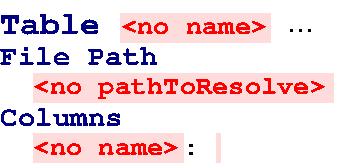
\includegraphics[width=\figWidthTiny]{figures/NewTable.pdf}
  \caption[New Table.]{\textbf{New Table.} This figure presents a freshly created Table AST Root node. You can use the button located to the right, after the <no name> red label (\keys{...}), to open a file selection dialog. Use this dialog to locate a TSV file to configure this table.}
\end{SCfigure}\label{fig:NewTable}

Figure~\ref{fig:ExampleTable} presents a MetaR table annotated with groups. 

\begin{figure}[h!tbp]
  \centering
  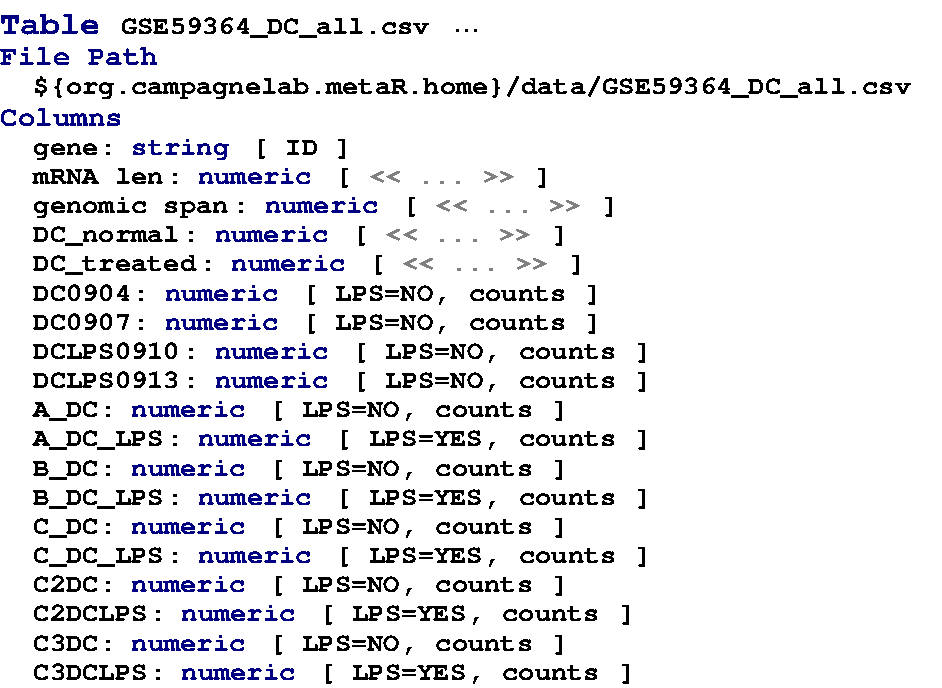
\includegraphics[width=\figWidthWide]{figures/ExampleTable.pdf}
\caption[Example Table.]{\textbf{Example Table.} The figure presents an example table annotated with groups.}
\label{fig:ExampleTable}
\end{figure}


\section{Column Groups Container}\label{sec:ColumnGroupContainer}\index{Column Groups Container}
Column Groups Container are used to define column groups and annotate these groups with group usages.
To create a new Column Group Container, right-click on a model and select \menu{New > o.c.tables.ColumnGroupContainer}. This will create the empty container shown in Figure~\ref{fig:NewColumnGroupContainer}. You need and should have only one container per model. The container will hold the groups and group usages that you need across one or more MetaR Tables.
\begin{SCfigure}
  \centering
  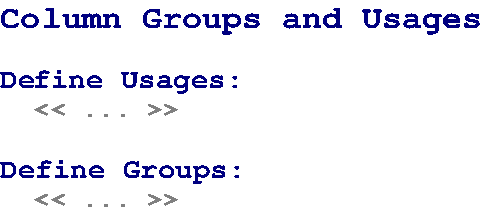
\includegraphics[width=\figWidthNarrow]{figures/NewColumnGroupContainer.pdf}
\caption[Empty Column Group Container.]{\textbf{Empty Column Group Container.} Use a column group container to define column groups and associated group usages. Place the cursor over the \mpsplaceholder{} symbol and press \keys{\return} to add a new group or group usage. Name the group or usage immediately after creating it.}
\label{fig:NewColumnGroupContainer}
\end{SCfigure}

\section{Column Groups}\index{Column Groups}
Column Groups can be defined by pressing \keys{\return} either on top of the \mpsplaceholder{} (immediately below \texttt{Define Groups:}), when the list of groups is empty, or with the cursor immediately before the name of an existing group. Each group has a name and an optional set of group usages. Figure~\ref{fig:NewGroup} presents a new column group (group for short).

\begin{SCfigure}
  \centering
  
\includegraphics[width=\figWidthNarrow]{figures/NewGroup.pdf}
\caption[New Group.]{\textbf{New Group.} You should name a new group immediately after creating it.}
\label{fig:NewGroup}
\end{SCfigure}

\paragraph{name} The name of the group is a string that should mean something in the context of your analysis. Some MetaR analysis statements require specific group names to be defined in a model container and referenced in an input table. Other groups will be created by you with meaningful names to help identify columns that have certain properties, so that you can refer to them collectively by the group name. 

\paragraph{used for}
Column groups can be annotated with a set of group usages. You can enter references to usages already defined in the column group container following the \texttt{used for} keyword shown in Figure~\ref{fig:NewGroup}. Press \keys{\enter} on the \mpsplaceholder{} to insert the first group usage. Make sure the usage is defined (its name should be visible in the \texttt{Define Usages:} section of the container (see Section~\ref{sec:ColumnGroupUsage} to lean how to create a new Group Usage). You can bind a group usage reference to a Group usage by using auto-completion (\keys{\ctrl+\space} to locate the name, then pressing \keys{\enter} to accept one completion choice), or by typing the name of the group usage directly (note that group usage names are case sensitive).

\begin{remark}
	Pressing \keys{\return} before \texttt{<no name>} will not have the desired effect if you have not yet named a group. Make sure you name groups immediately after you create them. 
\end{remark}

 
\section{Column Group Usage}\label{sec:ColumnGroupUsage}
A Column Group Usage can be defined by pressing \keys{\return} either on top of the \mpsplaceholder{} (immediately below \texttt{Define Usages:}), when the list of group usages is empty, or with the cursor immediately before the name of an existing group usage. When the list already contains one or more group usages, you can add more by placing the cursor over a group usage name and pressing \keys{\enter}. Keep pressing \keys{\enter} to add more empty group usages.

\section{Example Column Group Container}
Figure~\ref{fig:ExampleGroupContainer} presents an example of a configured Column Group Container. This container defines two groups \texttt{LPS=yes} and \texttt{LPS=no}, which can be used to annotate Table columns that contain data about gene expression of samples treated with LPS or not.  The group usage \texttt{LPS\_Treatment} is associated to both groups to indicate that they belong together and are two kinds of treatment.

\begin{SCfigure}
  \centering
  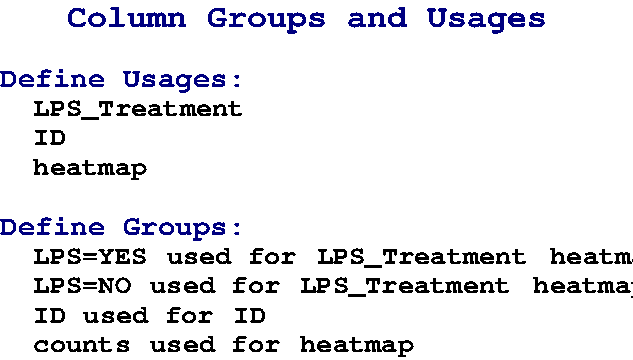
\includegraphics[width=\figWidthNarrow]{figures/ExampleGroupContainer.pdf}
\caption[Example Group Container.]{\textbf{Example Group Container.} This example presents a container with several groups and group usages.}
\label{fig:ExampleGroupContainer}
\end{SCfigure}
